\chapter{Nghiệm của phương trình một ẩn}
Trong nhiều lĩnh vực khoa học và kỹ thuật, việc giải phương trình phi tuyến đóng vai trò quan trọng. 
Một ví dụ tiêu biểu là mô hình tăng trưởng dân số, trong đó tốc độ tăng trưởng tỉ lệ thuận với quy mô hiện tại của quần thể. 
Khi bổ sung thêm yếu tố nhập cư với tốc độ hằng, ta thu được phương trình vi phân phức tạp hơn. 
Xét trường hợp một cộng đồng có dân số ban đầu $N(0) = 1{,}000{,}000$, sau một năm có thêm $435{,}000$ người nhập cư và tổng dân số đạt $N(1) = 1{,}564{,}000$. 
Để xác định tỉ lệ sinh $\lambda$, ta cần giải phương trình

\[
1{,}564{,}000 \;=\; 1{,}000{,}000 e^{\lambda} + \frac{435{,}000}{\lambda}\big(e^{\lambda} - 1\big).
\]

Rõ ràng phương trình này không thể giải chính xác bằng các phương pháp đại số thông thường. 
Trong những tình huống như vậy, các kỹ thuật số trở thành công cụ thiết yếu, cho phép tìm nghiệm xấp xỉ với độ chính xác tùy ý. 

Mục tiêu của Chương 2 là trình bày và phân tích một số phương pháp số cơ bản để giải các phương trình một biến, 
bao gồm \textit{phương pháp chia đôi}, \textit{lặp điểm cố định}, \textit{Newton--Raphson} và \textit{Secant}. 
Những phương pháp này không chỉ minh họa cách tiếp cận bài toán nghiệm phi tuyến, 
mà còn cho thấy sức mạnh của tính toán số trong việc giải quyết các phương trình mà giải tích không xử lý được.

\section{Phương pháp chia đổi (The Bisection Method)}

Một trong những kỹ thuật cơ bản nhất để giải phương trình phi tuyến $f(x) = 0$ là 
\textit{phương pháp chia đôi} (Bisection Method). 
Ý tưởng dựa trên \textit{Định lý Giá trị Trung gian}: 
nếu $f$ liên tục trên khoảng $[a,b]$ và $f(a)f(b) < 0$, 
thì tồn tại ít nhất một nghiệm $p \in (a,b)$ sao cho $f(p) = 0$.  

Phương pháp tiến hành như sau:  
bắt đầu với khoảng $[a,b]$, ta tính trung điểm
\[
p = \frac{a+b}{2}.
\]
Nếu $f(p) = 0$, nghiệm đã được tìm thấy. 
Ngược lại, tùy thuộc vào dấu của $f(p)$, ta chọn nửa khoảng chứa nghiệm:  
\[
[a,p] \quad \text{nếu } f(a)f(p)<0, 
\qquad \text{hoặc} \qquad
[p,b] \quad \text{nếu } f(p)f(b)<0.
\]
Quy trình này được lặp lại cho đến khi khoảng có độ dài nhỏ hơn sai số cho phép $\text{TOL}$.

\begin{figure}[h!]
\centering
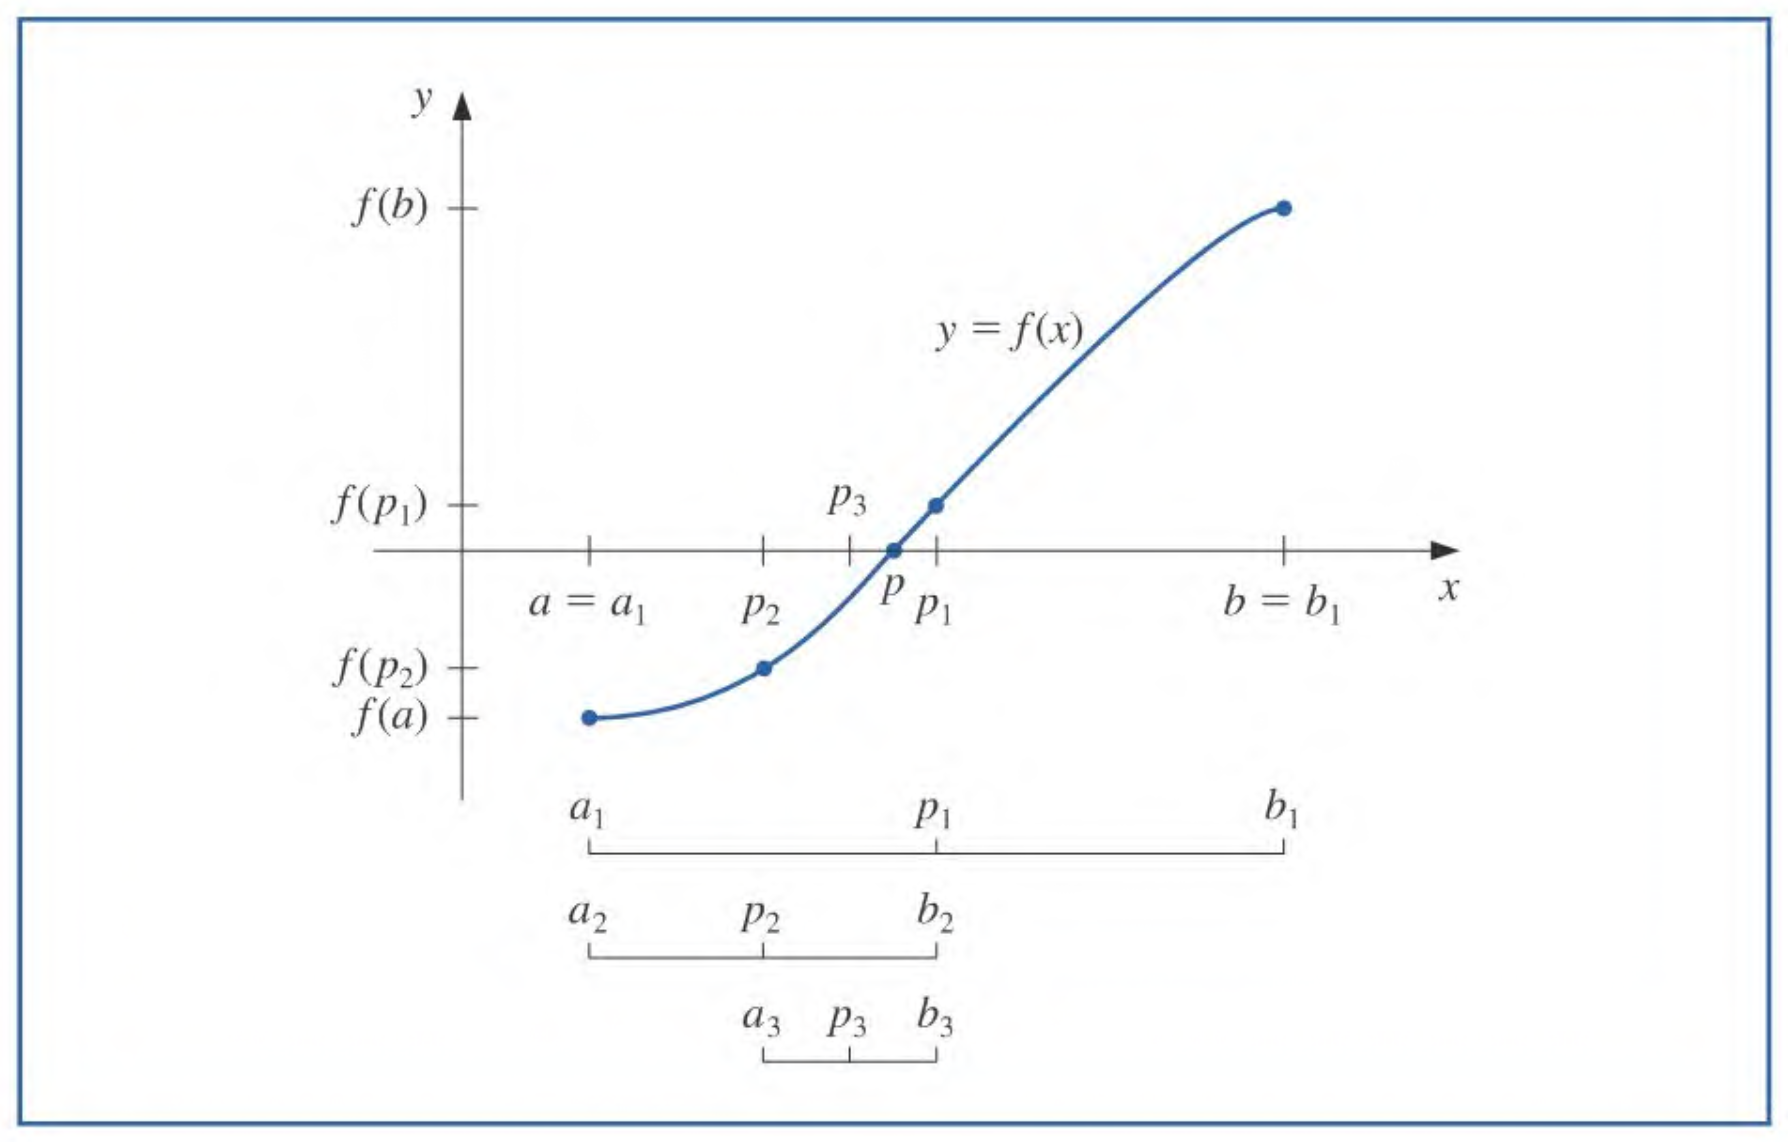
\includegraphics[width=0.7\textwidth]{assets/figure2.1.png}
\caption{Minh họa phương pháp chia đôi (Figure 2.1).}
\label{fig:bisection-fig21}
\end{figure}

\subsection*{\textbf{Thuật toán (Bisection Method)}}

\begin{enumerate}
    \item Chọn $a, b$ sao cho $f(a)f(b)<0$, cùng số lần lặp tối đa $N$ và sai số $\text{TOL}$.
    \item Với $i=1,2,\dots,N$:
    \begin{enumerate}
        \item Tính $p = \tfrac{a+b}{2}$.
        \item Nếu $|f(p)| < \text{TOL}$ hoặc $\tfrac{b-a}{2} < \text{TOL}$, kết thúc và nhận $p$ là nghiệm gần đúng.
        \item Nếu $f(a)f(p)>0$, đặt $a=p$; ngược lại, đặt $b=p$.
    \end{enumerate}
\end{enumerate}

Nếu sau $N$ bước mà chưa đạt điều kiện dừng, thuật toán được xem là thất bại.

\subsection*{\textbf{Ví dụ 1: Phương pháp chia đôi}}

Chứng minh rằng phương trình
\[
f(x) = x^3 + 4x^2 - 10 = 0
\]
có nghiệm trong khoảng $[1,2]$, và sử dụng phương pháp chia đôi để tìm nghiệm xấp xỉ với độ chính xác ít nhất $10^{-4}$.

\textbf{Lời giải.}  
Vì $f(1) = -5 < 0$ và $f(2) = 14 > 0$, nên theo Định lý Giá trị Trung gian, tồn tại ít nhất một nghiệm trong $[1,2]$.  

Ở lần lặp đầu tiên, $p_1 = 1.5$ và $f(1.5) = 2.375 > 0$, do đó nghiệm thuộc khoảng $[1,1.5]$.  
Tiếp tục chia đôi, $p_2 = 1.25$ với $f(1.25) = -1.7969 < 0$, nên nghiệm nằm trong $[1.25,1.5]$.  
Lặp lại quá trình này, ta thu được các giá trị trong Bảng~1.1.

\begin{center}
\captionof{table}{Các bước của phương pháp chia đôi cho $f(x) = x^3 + 4x^2 - 10$}
\begin{tabular}{|c|c|c|c|c|}
\hline
$n$ & $a_n$ & $b_n$ & $p_n$ & $f(p_n)$ \\
\hline
1  & 1.0000 & 2.0000 & 1.5000 & 2.3750 \\
2  & 1.0000 & 1.5000 & 1.2500 & -1.7969 \\
3  & 1.2500 & 1.5000 & 1.3750 & 0.1621 \\
4  & 1.2500 & 1.3750 & 1.3125 & -0.8484 \\
5  & 1.3125 & 1.3750 & 1.3438 & -0.3510 \\
6  & 1.3438 & 1.3750 & 1.3594 & -0.0964 \\
7  & 1.3594 & 1.3750 & 1.3672 & 0.0324 \\
8  & 1.3594 & 1.3672 & 1.3633 & -0.0322 \\
9  & 1.3633 & 1.3672 & 1.3652 & 0.000072 \\
10 & 1.3633 & 1.3652 & 1.3643 & -0.01605 \\
11 & 1.3643 & 1.3652 & 1.3647 & -0.00799 \\
12 & 1.3647 & 1.3652 & 1.3650 & -0.00396 \\
13 & 1.3650 & 1.3652 & 1.3651 & -0.00194 \\
\hline
\end{tabular}
\end{center}

Sau 13 lần lặp, ta được nghiệm xấp xỉ
\[
p_{13} = 1.365112305,
\]
với sai số
\[
|p - p_{13}| < |p_{14} - p_{13}| = |1.365234375 - 1.365112305| = 0.00012207,
\]
nên đảm bảo chính xác ít nhất $10^{-4}$.  
Giá trị đúng của nghiệm (chính xác đến 9 chữ số thập phân) là
\[
p = 1.365230013.
\]

\subsection*{\textbf{Định lý}}

Giả sử $f$ là hàm liên tục trên đoạn $[a,b]$ và thỏa $f(a)f(b) < 0$.  
Khi áp dụng phương pháp chia đôi, ta thu được một dãy $\{p_n\}_{n=1}^\infty$ hội tụ về nghiệm $p$ của $f(x)=0$.  
Hơn nữa, sai số tại bước lặp thứ $n$ được ước lượng bởi
\[
|p_n - p| < \frac{b-a}{2^n}, \quad n \geq 1.
\]

\textbf{Hệ quả.}  
Dãy $\{p_n\}$ hội tụ về $p$ với tốc độ $O(2^{-n})$, tức là
\[
p_n = p + O(2^{-n}).
\]

\subsection*{\textbf{Ví dụ 2: Ước lượng số lần lặp}}

Xác định số lần lặp cần thiết để giải phương trình
\[
f(x) = x^3 + 4x^2 - 10 = 0
\]
với độ chính xác $10^{-3}$, sử dụng $a_1 = 1$ và $b_1 = 2$.

\textbf{Lời giải.}  
Theo Định lý, sai số sau $N$ lần lặp thỏa
\[
|p_N - p| \leq \frac{b-a}{2^N}.
\]
Với $a=1, b=2$, ta có
\[
|p_N - p| \leq \frac{1}{2^N}.
\]

Để đạt độ chính xác $10^{-3}$, cần
\[
\frac{1}{2^N} \leq 10^{-3}
\quad \Rightarrow \quad
N \geq \frac{3}{\log_{10} 2} \approx 9.96.
\]

Vậy cần ít nhất $N=10$ lần lặp để đảm bảo nghiệm gần đúng nằm trong sai số $10^{-3}$.



\section{Fixed-Point Iteration}




\section{Phương pháp Newton và các mở rộng}

Isaac Newton (1643–1727) là một trong những nhà khoa học vĩ đại nhất mọi thời đại. 
Vào cuối thế kỷ 17, các công trình của ông đã chạm đến hầu hết các lĩnh vực toán học. 
Phương pháp mang tên ông được giới thiệu nhằm tìm nghiệm của phương trình
\[
y^3 - 2y - 5 = 0.
\]
Mặc dù Newton minh hoạ phương pháp chủ yếu cho đa thức, ông đã nhận ra khả năng ứng dụng rộng hơn của nó.

Phương pháp Newton (Newton--Raphson) là một trong những kỹ thuật số mạnh mẽ và nổi tiếng để tìm nghiệm của phương trình phi tuyến. 
Có nhiều cách trình bày phương pháp: (i) trực quan bằng hình học/đồ thị như trong giải tích; 
(ii) như một lược đồ có tốc độ hội tụ nhanh hơn so với một số lặp hàm khác; 
và (iii) dựa trên khai triển Taylor, vừa dẫn ra công thức, vừa cho phép ước lượng sai số xấp xỉ. 
Dưới đây là cách suy ra công thức bằng khai triển Taylor.

Giả sử $f \in C^2[a,b]$. Cho $p_0 \in [a,b]$ là một xấp xỉ ban đầu của nghiệm $p$ sao cho $f'(p_0) \neq 0$ và $|p - p_0|$ ``nhỏ''. 
Khai triển Taylor bậc nhất của $f$ tại $x=p_0$, đánh giá ở $x=p$, cho
\[
f(p) \;=\; f(p_0) + (p - p_0)\,f'(p_0) + \tfrac{1}{2} f''(\xi)\,(p - p_0)^2,
\]
với một $\xi$ nằm giữa $p$ và $p_0$. 
Vì $f(p)=0$, ta được
\[
0 \;=\; f(p_0) + (p - p_0)\,f'(p_0) + \tfrac{1}{2} f''(\xi)\,(p - p_0)^2.
\]
Nếu $|p - p_0|$ đủ nhỏ, bỏ qua hạng bậc hai cho xấp xỉ tuyến tính
\[
0 \;\approx\; f(p_0) + (p - p_0)\,f'(p_0),
\]
từ đó
\[
p \;\approx\; p_0 - \frac{f(p_0)}{f'(p_0)}.
\]

Suy ra công thức truy hồi Newton
\[
p_{n} \;=\; p_{n-1} - \frac{f(p_{n-1})}{f'(p_{n-1})}, \qquad n \ge 1. \tag{2.7}
\]

% (Tuỳ chọn) Hình minh hoạ tiếp tuyến:
% \begin{figure}[h!]
% \centering
% \includegraphics[width=0.6\textwidth]{figure_newton_tangent.png}
% \caption{Minh hoạ phương pháp Newton: từ $p_0$, lấy giao điểm trục hoành của tiếp tuyến tại $(p_0, f(p_0))$ để được $p_1$, rồi lặp.}
% \label{fig:newton-geom}
% \end{figure}

\subsection*{\textbf{Thuật toán – Phương pháp Newton}}

INPUT: giá trị gần đúng ban đầu $p_0$, sai số cho phép \texttt{TOL}, số lần lặp tối đa $N_0$.  

OUTPUT: nghiệm gần đúng $p$, hoặc thông báo thất bại.

\begin{enumerate}
  \item Đặt $i = 1$.
  \item Trong khi $i \leq N_0$, thực hiện:
  \begin{enumerate}
    \item Tính
    \[
    p = p_0 - \frac{f(p_0)}{f'(p_0)}.
    \]
    \item Nếu $|p - p_0| < \texttt{TOL}$, thì xuất $p$ và \textbf{STOP}.
    \item Đặt $i = i+1$, $p_0 = p$.
  \end{enumerate}
  \item Nếu chưa hội tụ sau $N_0$ bước, xuất thông báo: ``Phương pháp thất bại sau $N_0$ lần lặp.'' và \textbf{STOP}.
\end{enumerate}

\subsection*{Điều kiện dừng và dạng lặp của phương pháp Newton}

Các bất đẳng thức dừng được dùng trong phương pháp chia đôi cũng có thể áp dụng cho phương pháp Newton. 
Cụ thể, chọn một ngưỡng sai số $\varepsilon > 0$ và xây dựng dãy $\{p_n\}$ cho đến khi đạt một trong các điều kiện:

\[
|p_N - p_{N-1}| < \varepsilon \tag{2.8}
\]

\[
\frac{|p_N - p_{N-1}|}{|p_N|} < \varepsilon, 
\quad p_N \neq 0 \tag{2.9}
\]

hoặc

\[
|f(p_N)| < \varepsilon. \tag{2.10}
\]

Một dạng của (2.8) thường được sử dụng ở bước 4 trong Thuật toán 2.3. 
Lưu ý rằng không bất đẳng thức nào trong (2.8)--(2.10) cung cấp thông tin chính xác về sai số thực sự $|p_N - p|$.

Phương pháp Newton cũng có thể được xem như một dạng lặp điểm cố định, với công thức
\[
p_n = g(p_{n-1}) = p_{n-1} - \frac{f(p_{n-1})}{f'(p_{n-1})}, \quad n \geq 1. \tag{2.11}
\]

Đây chính là dạng lặp đã mang lại sự hội tụ rất nhanh được quan sát ở cột (e) trong Bảng~\ref{tab:fixedpoint-table}. 
Tuy nhiên, phương pháp không thể tiếp tục nếu $f'(p_{n-1}) = 0$ tại một bước nào đó. 
Trên thực tế, phương pháp Newton hiệu quả nhất khi $f'$ không tiến gần 0 trong một lân cận của nghiệm $p$.

\subsection*{\textbf{Ví dụ 1}}

Xét hàm $f(x) = \cos x - x$. Hãy xấp xỉ nghiệm của $f$ bằng:
\begin{enumerate}[label=(\alph*)]
  \item phương pháp lặp điểm cố định;
  \item phương pháp Newton.
\end{enumerate}

\textbf{Lời giải.}

(a) Nghiệm của bài toán tìm nghiệm cũng chính là nghiệm của bài toán điểm cố định $x = \cos x$. 
Đồ thị trong Hình~\ref{fig:fixedpoint-cosx} cho thấy có đúng một điểm cố định $p$ trong khoảng $[0,\tfrac{\pi}{2}]$. 

Với giá trị khởi đầu $p_0 = \pi/4$, ta thu được kết quả ở Bảng~\ref{tab:fixedpoint-cosx}.

\begin{center}
\captionof{table}{Lặp điểm cố định cho $f(x) = \cos x - x$, $p_0 = \pi/4$}
\label{tab:fixedpoint-cosx}
\begin{tabular}{|c|c|}
\hline
$n$ & $p_n$ \\
\hline
0 & 0.7853981635 \\
1 & 0.7071067810 \\
2 & 0.7602445972 \\
3 & 0.7246674808 \\
4 & 0.7487198858 \\
5 & 0.7325608446 \\
6 & 0.7434642113 \\
7 & 0.7361282565 \\
\hline
\end{tabular}
\end{center}

Từ bảng trên, có thể kết luận nghiệm $p \approx 0.74$.

(b) Để áp dụng phương pháp Newton, ta có
\[
f'(x) = -\sin x - 1.
\]

Với $p_0 = \pi/4$, lần lượt tính được:
\[
p_1 = p_0 - \frac{\cos(\pi/4) - \pi/4}{-\sin(\pi/4) - 1} \approx 0.7395361337,
\]
\[
p_2 = p_1 - \frac{\cos(p_1) - p_1}{-\sin(p_1) - 1} \approx 0.7390851781,
\]
\[
p_3 = p_2 - \frac{\cos(p_2) - p_2}{-\sin(p_2) - 1} \approx 0.7390851332.
\]

Kết quả được trình bày trong Bảng~\ref{tab:newton-cosx}.

\begin{center}
\captionof{table}{Phương pháp Newton cho $f(x) = \cos x - x$, $p_0 = \pi/4$}
\label{tab:newton-cosx}
\begin{tabular}{|c|c|}
\hline
$n$ & $p_n$ \\
\hline
0 & 0.7853981635 \\
1 & 0.7395361337 \\
2 & 0.7390851781 \\
3 & 0.7390851332 \\
4 & 0.7390851332 \\
\hline
\end{tabular}
\end{center}

Chỉ sau ba bước lặp, nghiệm gần đúng đã đạt $p \approx 0.7390851332$, 
chính xác hơn nhiều so với bảy bước lặp điểm cố định.

\subsection*{Hội tụ khi dùng phương pháp Newton}

Ví dụ 1 đã cho thấy phương pháp Newton có thể tạo ra xấp xỉ cực kỳ chính xác chỉ với rất ít bước lặp. 
Trong ví dụ đó, chỉ một lần lặp Newton đã cho độ chính xác tốt hơn bảy lần lặp bằng phương pháp điểm cố định. 
Bây giờ, ta sẽ xem xét kỹ hơn để hiểu tại sao Newton lại hiệu quả như vậy.

Khai triển Taylor ở đầu mục 2.3 đã chỉ ra tầm quan trọng của việc chọn gần đúng ban đầu chính xác. 
Giả định then chốt là số hạng bậc hai $(p - p_0)^2$ nhỏ hơn nhiều so với $|p - p_0|$, 
nên có thể bỏ qua. Điều này rõ ràng không đúng trừ khi $p_0$ đủ gần nghiệm $p$. 
Nếu $p_0$ không đủ gần nghiệm thực sự, thì khó có lý do để tin rằng Newton sẽ hội tụ về nghiệm. 
Tuy nhiên, trong một số trường hợp, ngay cả những xấp xỉ ban đầu kém cũng có thể dẫn đến hội tụ 
(xem thêm các Bài tập 15 và 16).

Định lý sau đây làm sáng tỏ sự hội tụ của phương pháp Newton và nhấn mạnh tầm quan trọng 
của việc chọn giá trị khởi đầu $p_0$.

\subsection*{Định lý (Hội tụ của phương pháp Newton)}

Giả sử $f \in C^2[a,b]$. Nếu $p \in (a,b)$ thỏa mãn $f(p)=0$ và $f'(p) \neq 0$, 
thì tồn tại một $\delta > 0$ sao cho phương pháp Newton sinh ra dãy 
$\{p_n\}_{n=1}^\infty$ hội tụ về $p$ với mọi giá trị khởi đầu 
$p_0 \in [p-\delta,\, p+\delta]$.

\textbf{Phác thảo chứng minh.}  
Xem phương pháp Newton như một lặp điểm cố định:
\[
p_n = g(p_{n-1}), \quad n \geq 1,
\]
trong đó
\[
g(x) = x - \frac{f(x)}{f'(x)}.
\]

Ta cần tìm một khoảng $[p-\delta,\,p+\delta]$ sao cho $g$ ánh xạ khoảng này vào chính nó 
và tồn tại hằng số $k < 1$ sao cho $|g'(x)| \leq k$ trên đó.

Vì $f'(p) \neq 0$ và $f \in C^2$, nên $g$ khả vi và liên tục trong một lân cận của $p$. 
Hơn nữa,
\[
g'(p) = \frac{f(p)f''(p)}{[f'(p)]^2} = 0,
\]
vì $f(p) = 0$. Do đó, tồn tại $\delta > 0$ sao cho $|g'(x)| < k < 1$ 
với mọi $x \in [p-\delta,\,p+\delta]$.

Theo Định lý điểm cố định, dãy $\{p_n\}$ sẽ hội tụ đến điểm cố định $p$.

\section*{\textbf{The Secant Method}}

Phương pháp Newton là một kỹ thuật rất mạnh, nhưng có một nhược điểm lớn: 
cần biết giá trị của đạo hàm $f'(x)$ tại mỗi bước lặp. 
Trong nhiều trường hợp, việc tính đạo hàm còn khó khăn và tốn nhiều phép tính hơn so với tính $f(x)$.

Để khắc phục vấn đề này, ta xét một biến thể: thay vì sử dụng $f'(p_{n-1})$, 
ta xấp xỉ nó bằng công thức sai phân
\[
f'(p_{n-1}) \;\approx\; \frac{f(p_{n-1}) - f(p_{n-2})}{p_{n-1} - p_{n-2}}.
\]

Thay vào công thức Newton, ta thu được
\[
p_n \;=\; p_{n-1} - f(p_{n-1}) \cdot \frac{p_{n-1} - p_{n-2}}{f(p_{n-1}) - f(p_{n-2})}, 
\qquad n > 1. \tag{2.12}
\]

Kỹ thuật này được gọi là \textit{phương pháp Secant} và được mô tả trong Thuật toán 2.4.

Phương pháp bắt đầu với hai giá trị khởi đầu $p_0$ và $p_1$. 
Nghiệm gần đúng $p_2$ chính là giao điểm với trục hoành của đường secant đi qua hai điểm 
$(p_0, f(p_0))$ và $(p_1, f(p_1))$. 
Sau đó, $p_3$ được tính bằng giao điểm của secant nối $(p_1, f(p_1))$ và $(p_2, f(p_2))$, 
và tiếp tục như vậy. 

Điểm quan trọng là, sau khi tính $f(p_0)$ và $f(p_1)$, 
mỗi bước của phương pháp Secant chỉ cần thêm một phép tính giá trị hàm số. 
Trong khi đó, mỗi bước của Newton yêu cầu cả $f$ và $f'$. 
Vì vậy, trong nhiều trường hợp phương pháp Secant là một lựa chọn kinh tế hơn.

---

\subsection*{\textbf{Thuật toán – Phương pháp Secant}}

INPUT: hai giá trị khởi đầu $p_0, p_1$, sai số cho phép \texttt{TOL}, số lần lặp tối đa $N_0$.  

OUTPUT: nghiệm gần đúng $p$, hoặc thông báo thất bại.

\begin{enumerate}
  \item Đặt $i = 2$.
  \item Trong khi $i \leq N_0$, thực hiện:
  \begin{enumerate}
    \item Tính
    \[
    p = p_{i-1} - f(p_{i-1}) \cdot \frac{p_{i-1} - p_{i-2}}{f(p_{i-1}) - f(p_{i-2})}.
    \]
    \item Nếu $|p - p_{i-1}| < \texttt{TOL}$, thì xuất $p$ và \textbf{STOP}.
    \item Đặt $i = i+1$, $p_{i-2} = p_{i-1}$, $p_{i-1} = p$.
  \end{enumerate}
  \item Nếu chưa hội tụ sau $N_0$ bước, xuất thông báo: 
  ``Phương pháp thất bại sau $N_0$ lần lặp.'' và \textbf{STOP}.
\end{enumerate}

\subsection*{\textbf{Phương pháp dây cung}}

Phương pháp Secant có thể hội tụ nhanh hơn phương pháp Newton trong một số trường hợp, 
nhưng nó không đảm bảo giữ nghiệm xấp xỉ trong khoảng ban đầu $[a,b]$. 
Nếu $f(a)$ và $f(b)$ trái dấu, phương pháp dây cung (\textit{method of false position}, 
hay \textit{Regula Falsi}) vừa tận dụng ý tưởng secant vừa giữ được tính chất 
“bracketing” như phương pháp chia đôi.

Ý tưởng cơ bản là: bắt đầu với $a_0$ và $b_0$ sao cho $f(a_0)f(b_0) < 0$. 
Xác định $p_0$ là giao điểm trục hoành của đường secant qua $(a_0,f(a_0))$ và $(b_0,f(b_0))$, tức là
\[
p_0 = b_0 - f(b_0)\,\frac{b_0 - a_0}{f(b_0) - f(a_0)}.
\]

Nếu $f(p_0) = 0$ thì $p_0$ chính là nghiệm. 
Nếu không, ta chọn cặp khoảng mới $[a_1,b_1]$ sao cho $f(a_1)f(b_1)<0$, 
trong đó một đầu mút là $p_0$ và đầu mút còn lại được giữ từ bước trước. 
Tiếp tục quá trình để thu được dãy $\{p_n\}$.

\textbf{Thuật toán – Phương pháp dây cung}

INPUT: $a$, $b$ sao cho $f(a)f(b)<0$; sai số cho phép \texttt{TOL}; số lần lặp tối đa $N_0$.  

OUTPUT: nghiệm gần đúng $p$, hoặc thông báo thất bại.

\begin{enumerate}
  \item Đặt $i = 1$.
  \item Trong khi $i \leq N_0$, thực hiện:
  \begin{enumerate}
    \item Tính
    \[
    p = b - f(b)\,\frac{b - a}{f(b) - f(a)}.
    \]
    \item Nếu $|f(p)| < \texttt{TOL}$, thì xuất $p$ và \textbf{STOP}.
    \item Nếu $f(a)f(p) < 0$, đặt $b = p$; ngược lại, đặt $a = p$.
    \item Đặt $i = i+1$.
  \end{enumerate}
  \item Nếu chưa hội tụ sau $N_0$ bước, xuất thông báo: 
  ``Phương pháp thất bại sau $N_0$ lần lặp.'' và \textbf{STOP}.
\end{enumerate}







\section{Phân tích sai số cho các phương pháp lặp (Error Analysis for Iterative Methods)}

Trong phần này, ta khảo sát \textit{bậc hội tụ} của các sơ đồ lặp hàm, 
từ đó rút ra phương pháp Newton như một công cụ để đạt hội tụ nhanh. 
Đồng thời, ta cũng xem xét các cách cải thiện tốc độ hội tụ của Newton trong một số trường hợp đặc biệt.

Trước hết, cần một khái niệm để đo tốc độ hội tụ của một dãy.

\subsection*{Định nghĩa 2.7 (Bậc hội tụ)}

Giả sử $\{p_n\}$ là một dãy hội tụ về $p$, với $p_n \neq p$ với mọi $n$. 
Nếu tồn tại các hằng số dương $\lambda$ và $\alpha$ sao cho
\[
\lim_{n \to \infty} \frac{|p_{n+1} - p|}{|p_n - p|^\alpha} = \lambda,
\]
thì ta nói dãy $\{p_n\}$ hội tụ về $p$ với \textbf{bậc $\alpha$}, 
và $\lambda$ được gọi là \textit{hằng số sai số tiệm cận}.

Một kỹ thuật lặp dạng $p_n = g(p_{n-1})$ được gọi là \textit{hội tụ bậc $\alpha$} 
nếu dãy $\{p_n\}$ hội tụ về nghiệm $p = g(p)$ với bậc $\alpha$.

Nói chung, bậc hội tụ càng cao thì dãy càng nhanh tiến tới nghiệm. 
Hằng số $\lambda$ cũng ảnh hưởng đến tốc độ, nhưng yếu tố quyết định là bậc $\alpha$. 
Hai trường hợp thường gặp:
\begin{enumerate}
  \item Nếu $\alpha = 1$ và $\lambda < 1$, dãy hội tụ tuyến tính (\textit{linear convergence}).
  \item Nếu $\alpha = 2$, dãy hội tụ bậc hai (\textit{quadratic convergence}).
\end{enumerate}

Ví dụ minh hoạ tiếp theo sẽ so sánh một dãy hội tụ tuyến tính với một dãy hội tụ bậc hai, 
cho thấy lý do tại sao nên tìm các phương pháp có bậc hội tụ cao.

\subsection*{\textbf{Minh hoạ}}

Giả sử $\{p_n\}$ là dãy hội tụ tuyến tính về $0$ với hằng số sai số tiệm cận $0.5$, tức là
\[
\lim_{n \to \infty} \frac{|p_{n+1}|}{|p_n|} = 0.5.
\]

Đồng thời, xét một dãy $\{q_n\}$ hội tụ bậc hai về $0$ với cùng hằng số sai số tiệm cận $0.5$, tức là
\[
\lim_{n \to \infty} \frac{|q_{n+1}|}{|q_n|^2} = 0.5.
\]

Với giả thiết $|p_0| = |q_0| = 1$, Bảng~\ref{tab:conv-rates} so sánh tốc độ hội tụ của hai dãy.

\begin{center}
\captionof{table}{So sánh tốc độ hội tụ tuyến tính và bậc hai}
\label{tab:conv-rates}
\begin{tabular}{|c|c|c|}
\hline
$n$ & Tuyến tính: $(0.5)^n$ & Bậc hai: $(0.5)^{2^n - 1}$ \\
\hline
1 & $5.0000 \times 10^{-1}$ & $5.0000 \times 10^{-1}$ \\
2 & $2.5000 \times 10^{-1}$ & $1.2500 \times 10^{-1}$ \\
3 & $1.2500 \times 10^{-1}$ & $7.8125 \times 10^{-3}$ \\
4 & $6.2500 \times 10^{-2}$ & $3.0518 \times 10^{-5}$ \\
5 & $3.1250 \times 10^{-2}$ & $4.6566 \times 10^{-10}$ \\
6 & $1.5625 \times 10^{-2}$ & $1.0842 \times 10^{-19}$ \\
7 & $7.8125 \times 10^{-3}$ & $5.8775 \times 10^{-39}$ \\
\hline
\end{tabular}
\end{center}

Ta thấy dãy hội tụ bậc hai đạt độ chính xác $10^{-38}$ chỉ sau 7 bước, 
trong khi dãy hội tụ tuyến tính cần ít nhất 126 bước để đạt cùng mức chính xác.


\subsection*{\textbf{Định lý 2.8}}

Giả sử $g \in C[a,b]$ và $g$ ánh xạ $[a,b]$ vào chính nó. 
Giả sử thêm rằng $g'$ liên tục trên $(a,b)$ và tồn tại hằng số $k < 1$ sao cho
\[
|g'(x)| \leq k, \quad \forall x \in (a,b).
\]

Nếu $g'(p) \neq 0$, thì với mọi giá trị khởi đầu $p_0 \neq p$ trong $[a,b]$, 
dãy
\[
p_n = g(p_{n-1}), \quad n > 1,
\]
hội tụ tuyến tính về nghiệm duy nhất $p \in [a,b]$, 
với hằng số sai số tiệm cận $|g'(p)|$.

\subsection*{\textbf{Định lý 2.9}}

Giả sử $p$ là nghiệm của phương trình $x = g(x)$. 
Nếu $g'(p) = 0$ và $g''$ liên tục với $|g''(x)| < M$ trên một khoảng mở $I$ chứa $p$, 
thì tồn tại $\delta > 0$ sao cho, với mọi $p_0 \in [p-\delta,\, p+\delta]$, 
dãy
\[
p_n = g(p_{n-1}), \quad n > 1,
\]
hội tụ ít nhất bậc hai đến $p$. Hơn nữa, với $n$ đủ lớn,
\[
|p_{n+1} - p| \;\leq\; \tfrac{M}{2}\,|p_n - p|^2.
\]


\subsection*{\textbf{Multiple Roots}}

Trong các phần trước, ta đã giả định rằng $f'(p) \neq 0$, 
với $p$ là nghiệm của phương trình $f(x) = 0$. 
Tuy nhiên, trong thực tế, khi $f'(p) = 0$ đồng thời với $f(p) = 0$, 
các phương pháp Newton và Secant thường gặp khó khăn. 
Để xem xét chi tiết hơn vấn đề này, ta đưa ra định nghĩa sau.

\subsection*{\textbf{Định nghĩa 2.10 (Nghiệm bội)}}

Một nghiệm $p$ của phương trình $f(x) = 0$ được gọi là 
\textit{nghiệm bội (zero of multiplicity)} bậc $m$ của $f$ 
nếu, với mọi $x \neq p$, ta có thể viết
\[
f(x) = (x - p)^m q(x),
\]
trong đó 
\[
\lim_{x \to p} q(x) \neq 0.
\]

Với đa thức, $p$ là nghiệm bội bậc $m$ của $f$ 
nếu $f(x) = (x - p)^m q(x)$ và $q(p) \neq 0$.

Về bản chất, $q(x)$ biểu diễn phần của hàm $f(x)$ 
không đóng góp vào nghiệm tại $x = p$. 
Kết quả tiếp theo sẽ giúp xác định các \textit{nghiệm đơn (simple zeros)}, 
tức là những nghiệm có bội bằng $1$.

\subsection*{\textbf{Định lý 2.11}}

Giả sử $f \in C^1[a,b]$. 
Hàm $f$ có \textit{nghiệm đơn (simple zero)} tại $p \in (a,b)$ 
khi và chỉ khi 
\[
f(p) = 0 \quad \text{và} \quad f'(p) \neq 0.
\]

\subsection*{\textbf{Định lý 2.12}}

Giả sử $f \in C^m[a,b]$.  
Hàm $f$ có nghiệm bội $m$ tại $p \in (a,b)$ 
khi và chỉ khi
\[
0 = f(p) = f'(p) = f''(p) = \cdots = f^{(m-1)}(p), 
\quad \text{nhưng} \quad f^{(m)}(p) \neq 0.
\]

Kết quả trong Định lý 2.12 cho thấy rằng 
nếu tồn tại một lân cận của $p$ mà tại đó phương pháp Newton được áp dụng, 
thì nó sẽ hội tụ bậc hai về $p$ đối với mọi giá trị khởi đầu $p_0$ đủ gần $p$, 
miễn là $p$ là nghiệm đơn.  
Ví dụ tiếp theo sẽ minh hoạ rằng hội tụ bậc hai có thể không xảy ra 
khi nghiệm không phải là nghiệm đơn.

\subsection*{Ví dụ 1 – Ảnh hưởng của nghiệm bội đến phương pháp Newton}

Xét hàm
\[
f(x) = e^x - x - 1.
\]

\begin{enumerate}[label=(\alph*)]
  \item Chứng minh rằng $f$ có nghiệm bội 2 tại $x = 0$.
  \item Áp dụng phương pháp Newton với $p_0 = 1$ để khảo sát tốc độ hội tụ.
\end{enumerate}

\textbf{Lời giải.}

(a)  
Ta có
\[
f'(x) = e^x - 1, 
\qquad 
f''(x) = e^x.
\]
Tại $x = 0$, ta nhận được
\[
f(0) = 0, 
\quad 
f'(0) = 0, 
\quad 
f''(0) = 1 \neq 0.
\]
Do đó, $x = 0$ là nghiệm bội 2 của $f(x)$.

(b)  
Áp dụng công thức Newton
\[
p_{n} = p_{n-1} - \frac{f(p_{n-1})}{f'(p_{n-1})}
       = p_{n-1} - \frac{e^{p_{n-1}} - p_{n-1} - 1}{e^{p_{n-1}} - 1}.
\]

Với $p_0 = 1$, ta thu được:
\[
\begin{aligned}
p_1 &= 1 - \frac{e - 2}{e - 1} 
      \approx 0.5819767, \\
p_2 &= 0.5819767 - 
      \frac{e^{0.5819767} - 0.5819767 - 1}{e^{0.5819767} - 1} 
      \approx 0.3190623, \\
p_3 &\approx 0.1729500, \\
p_4 &\approx 0.0906560, \\
p_5 &\approx 0.0460287.
\end{aligned}
\]

\begin{center}
\captionof{table}{Các giá trị lặp của phương pháp Newton cho $f(x)=e^x-x-1$}
\label{tab:newton-multroot}
\begin{tabular}{|c|c|}
\hline
$n$ & $p_n$ \\
\hline
0 & 1.0000000 \\
1 & 0.5819767 \\
2 & 0.3190623 \\
3 & 0.1729500 \\
4 & 0.0906560 \\
5 & 0.0460287 \\
\hline
\end{tabular}
\end{center}

Ta thấy dãy $\{p_n\}$ hội tụ đến nghiệm $p = 0$, 
nhưng tốc độ hội tụ chỉ là \textit{tuyến tính}, không phải bậc hai như trường hợp nghiệm đơn. 
Đây chính là hiện tượng chung của phương pháp Newton khi áp dụng cho các nghiệm bội.


\section{Accelerating Convergence}




